\chapter{Negocio}
\section{Introduccion}
Las descripciones arquitectónicas se centran en la estructura, lo que significa que las interrelaciones de las entidades dentro de una organización desempeñan un papel importante. Para hacerlo explícito, se ha introducido el elemento de la colaboración empresarial.\\

Se introduce el elemento de la interfaz empresarial para modelar explícitamente los lugares o canales (lógicos o físicos) en los que se puede acceder a los servicios que una función ofrece al entorno. El mismo servicio puede ofrecerse en varias interfaces diferentes; por ejemplo, por correo, por teléfono o a través de Internet. A diferencia de la modelización de aplicaciones, en los enfoques actuales de modelización de la capa empresarial no es frecuente reconocer el elemento de interfaz empresarial.
En la Capa de Negocio se definen tres tipos de elementos de estructura activa interna: actor comercial, papel comercial y colaboración comercial.\\

El aspecto de la estructura pasiva de la Capa de Negocios contiene los elementos de estructura pasiva (objetos de negocios) que son manipulados por el comportamiento, como los procesos o funciones de negocios. Las entidades pasivas representan los conceptos importantes en los que la empresa piensa en un dominio.
En la Capa de Negocios, hay dos tipos principales de elementos de estructura pasiva: objeto de negocio y representación. Además, un contrato, utilizado en el contexto de un producto, es una especialización de un objeto de negocio.

\newpage
\section{Metamodelo}

\begin{figure}[h!]
	\centering
	\begin{minipage}{1\textwidth} % choose width suitably
	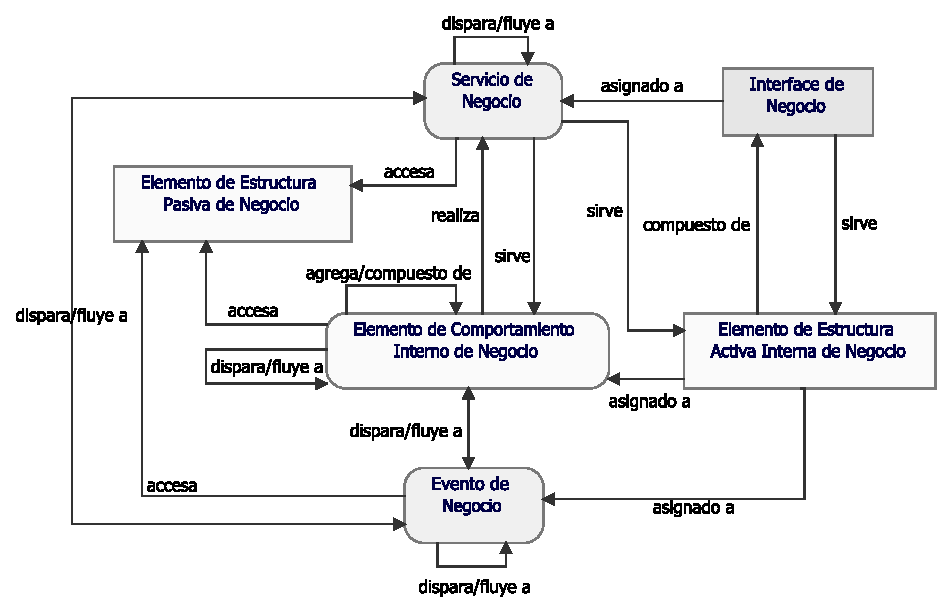
\includegraphics[width=0.9\linewidth]{imgs/meta/Negocio}
	\caption{Metamodelo Negocio}
	\label{fig:business}
	{\footnotesize Nota: Esta figura no muestra todas las relaciones permitidas; cada elemento del lenguaje puede tener relaciones de composición, agregación y especialización con elementos del mismo tipo; además, hay relaciones indirectas que pueden derivarse.\par}
	\end{minipage}
\end{figure}

La figura \ref{fig:business} ofrece una visión general de los elementos de la capa de negocios y sus relaciones. El elemento de estructura activa interna de la empresa, el elemento de comportamiento interno de la empresa y el elemento de estructura pasiva de la empresa son elementos abstractos; sólo sus especializaciones (como se definen en las siguientes secciones) se instancian en los modelos.

La Capa de Negocios se utiliza típicamente (a menudo en conjunto con los elementos de estrategia descritos en el Capítulo 5) para modelar la arquitectura de negocios de una empresa, definida por el marco del TOGAF como una descripción de la estructura e interacción entre la estrategia de negocios, la organización, las funciones, los procesos de negocios y las necesidades de información.

\newpage
\section{Punto de Vista de Organización}

El punto de vista de la organización se centra en la organización (interna) de una empresa, un departamento, una red de empresas o de otra entidad organizativa. Es posible presentar modelos en este punto de vista como diagramas de bloques anidados, pero también de una manera más tradicional, como los organigramas. El punto de vista de la organización es muy útil para identificar las competencias, la autoridad y las responsabilidades de una organización.

\subsection{Modelo de Organización}
\begin{figure}[h!]
	\centering
	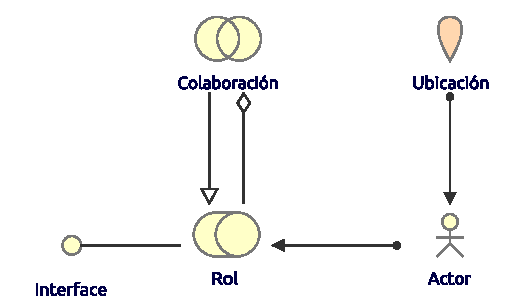
\includegraphics[width=.6\linewidth]{imgs/modelo/Organizacion}
	\caption{Modelo Organizacion}
\end{figure}

Un actor de negocios es una entidad de negocios que es capaz de realizar un comportamiento. Los actores pueden incluir entidades fuera de la organización real; por ejemplo, clientes y socios. Un actor comercial puede representar a esas entidades comerciales en diferentes niveles de detalle, y puede corresponder tanto a un actor como a una unidad organizativa en el marco del TOGAF. Ejemplos de actores comerciales son los seres humanos, los departamentos y las unidades comerciales. Una colaboración empresarial es un conjunto de dos o más elementos de la estructura activa interna de la empresa que trabajan juntos para llevar a cabo un comportamiento colectivo. Una interfaz de negocios es un punto de acceso en el que se pone a disposición del entorno un servicio comercial. Una interfaz comercial expone la funcionalidad de un servicio comercial a otros roles o actores comerciales. Se suele denominar canal (teléfono, Internet, oficina local, etc.). El mismo servicio comercial puede estar expuesto a través de diferentes interfaces.

\newpage
\subsection{Caso  de Organización}
\begin{figure}[h!]
	\centering
	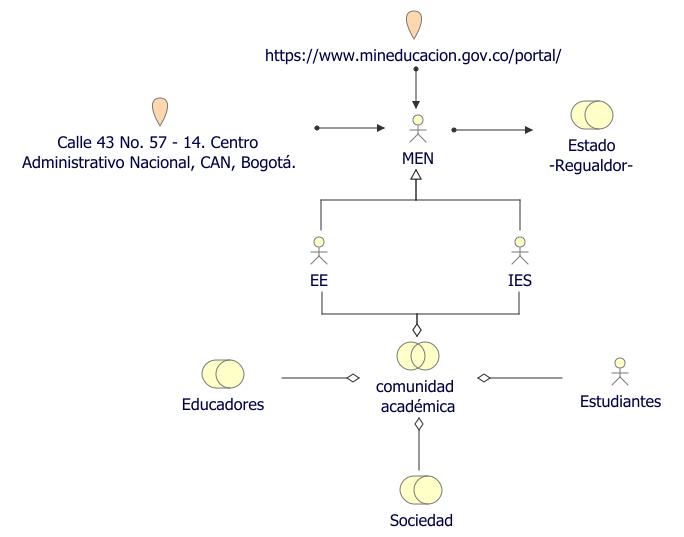
\includegraphics[width=.9\linewidth]{imgs/caso/negocio/organizacion}
	\caption{Caso Organizacion}
\end{figure}

El MEN tiene como actores principales los establecimientos educativos (EE), las instituciones de educación superior (IES) y las comunidades estudiantiles respectivas. Además, cuenta con ubicaciones tanto física como virtual, a saber, dispone de una dirección electrónica de dominio gubernamental como lo es \url{https://www.mineducacion.gov.co/portal/} y de una dirección física ubicada en la calle 43 No. 57 - 14 Centro 
Administrativo Nacional, CAN, Bogotá. Por otra parte, encontramos tres roles a destacar siendo el Estado uno de ellos y ejerciendo como ente regulador de las políticas a majear, así como, de emisor de recursos económicos junto con otro rol como lo es la sociedad y que, a su vez esta sociedad junto con el último de los roles a destacar, los educadores, colaboran o confluyen en una comunidad académica junto con los estudiantes, como otro de los actores principales de la organización.



\clearpage
\section{Punto de Vista de Cooperación de Actor}


\subsection{Modelo de Cooperación de Actor}
\begin{figure}[h!]
	\centering
	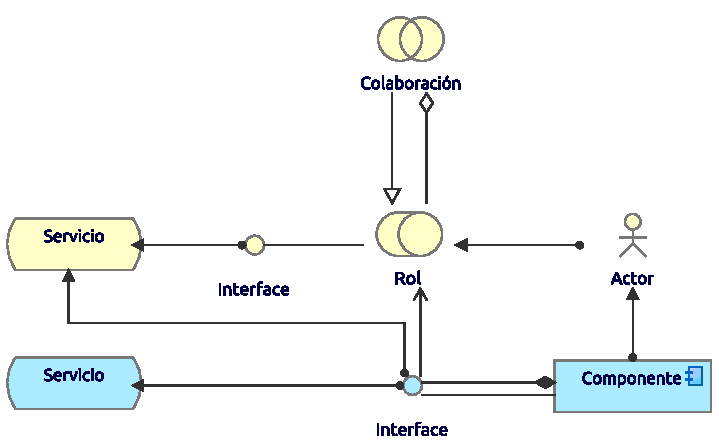
\includegraphics[width=.6\linewidth]{imgs/modelo/CoopActor.pdf}
	\caption{Modelo Cooperacion de Actor}
\end{figure}

El punto de vista de cooperación de actor establece las colaboraciones que existen internamente y externamente sobre un actor o rol de la organización con el fin de mostrar de qué manera interactuan e interfiere con el actor en cuestión. Por medio de interfaces  que comunican los entes del exterior y el interior de la organización con el actor o rol.

\newpage
\subsection{Caso  de Cooperación de Actor}
\begin{figure}[h!]
	\centering
	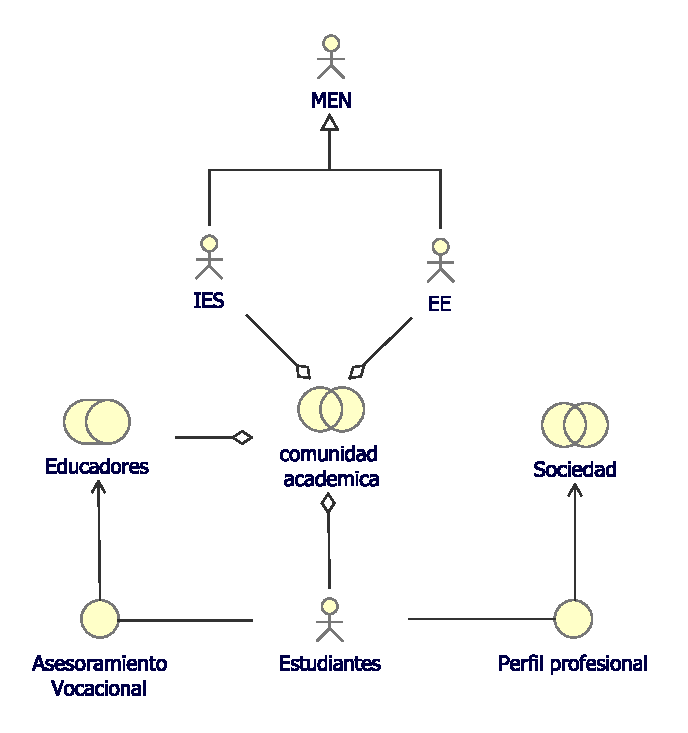
\includegraphics[width=.8\linewidth]{imgs/caso/negocio/coperacion_actor.pdf}
	\caption{Caso Cooperacion de Actor}
\end{figure}

Para nuestro objeto de estudio en relación al punto de vista de colaboración de actor tenemos como actor principal a los estudiantes aquellos que colaboran en la comunidad académica y hacen parte de las IES y EE que son regidas por el Ministerio de Educación. Por otro lado tenemos el rol de educador que hace parte de la comunidad y que puede ayudar a guiar en parte la vocación que construirá en un futuro el estudiante. Los estudiantes contribuirán en la sociedad gracias a su perfil que se ha formado durante sus años de estudio y que permitirán a las empresas apoderarse de estos individuos y así lograr mejores avances que colaboren en su entidad y por tanto a la sociedad misma.

\clearpage
\section{Punto de Vista de función de Negocio}

El punto de vista de la cooperación de los procesos comerciales se utiliza para mostrar las relaciones de uno o más procesos comerciales entre sí y/o con su entorno. Puede utilizarse tanto para crear un diseño de alto nivel de los procesos empresariales dentro de su contexto como para proporcionar a un director operacional responsable de uno o más de esos procesos una visión de sus dependencias. Los aspectos importantes de la cooperación en los procesos empresariales son:

\begin{itemize}
	\item Relaciones causales entre los principales procesos comerciales de la empresa
	\item Mapeo de los procesos comerciales en las funciones comerciales
	\item Realización de servicios por procesos comerciales
	\item Uso de datos compartidos
\end{itemize}

Cada una de ellas puede considerarse un "subpunto de vista" del punto de vista de la cooperación en los procesos comerciales.

\subsection{Modelo de función de Negocio}
\begin{figure}[h!]
	\centering
	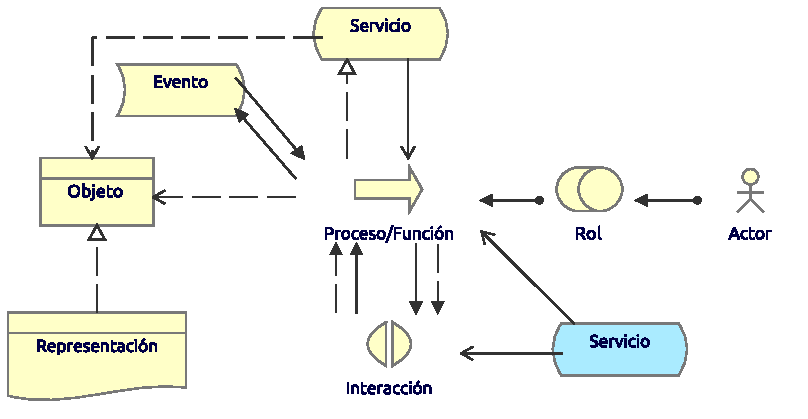
\includegraphics[width=.8\linewidth]{imgs/modelo/ProcesoNegocio}
	\caption{Modelo función de Negocio}
\end{figure}

Un proceso empresarial representa una secuencia de comportamientos empresariales que logra un resultado específico, como un conjunto definido de productos o servicios empresariales.
Un proceso de negocios describe el comportamiento interno realizado por un rol de negocios que se requiere para producir un conjunto de productos y servicios. Para un consumidor, los productos y servicios son relevantes y el comportamiento requerido es meramente una caja negra, de ahí la designación "interno".
Un proceso comercial complejo puede ser una agregación de otros procesos de grano más fino. A cada uno de ellos se le pueden asignar funciones más finas.
Existe una relación potencial de muchos a muchos entre los procesos de negocios y las funciones de negocios. En términos informales, los procesos describen algún tipo de "flujo" de actividades, mientras que las funciones agrupan las actividades según las aptitudes, los conocimientos, los recursos, etc. requeridos. Un proceso empresarial puede ser desencadenado por, o desencadenar, cualquier otro elemento de comportamiento empresarial (por ejemplo, un acto empresarial, un proceso empresarial, una función empresarial o una interacción empresarial). Un proceso empresarial puede acceder a objetos empresariales. Un proceso empresarial puede realizar uno o más servicios empresariales y pueden utilizar servicios comerciales (internos) o servicios de aplicación. Se puede asignar una función empresarial a un proceso empresarial para realizar este proceso manualmente. Un proceso empresarial automatizado puede realizarse mediante un proceso de aplicación. El nombre de un proceso empresarial debe indicar claramente una secuencia predefinida de acciones, y puede incluir la palabra "proceso". Ejemplos de ello son "adjudicar la reclamación", "incorporación de empleados", "proceso de aprobación" o "presentación de informes financieros". \\

Un objeto comercial representa un concepto utilizado dentro de un dominio comercial determinado. Un contrato representa una especificación formal o informal de un acuerdo entre un proveedor y un consumidor en el que se especifican los derechos y obligaciones asociados a un producto y se establecen parámetros funcionales y no funcionales para la interacción. Una representación representa una forma perceptible de la información que lleva un objeto comercial.

\clearpage
\subsection{Caso  de función de Negocio}
\begin{figure}[h!]
	\centering
	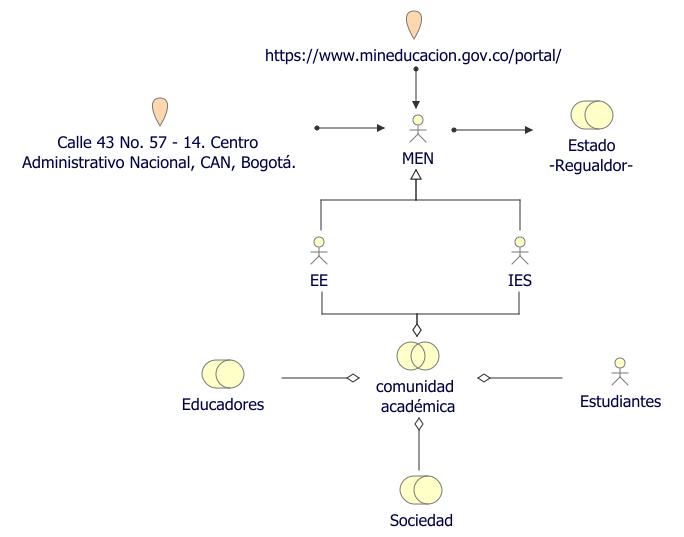
\includegraphics[width=.9\linewidth]{imgs/caso/negocio/organizacion}
	\caption{Caso función de Negocio}
\end{figure}
descripcion...


\clearpage
\section{Punto de Vista de Proceso de Negocio}

El punto de vista de la cooperación de los procesos comerciales se utiliza para mostrar las relaciones de uno o más procesos comerciales entre sí y/o con su entorno. Puede utilizarse tanto para crear un diseño de alto nivel de los procesos empresariales dentro de su contexto como para proporcionar a un director operacional responsable de uno o más de esos procesos una visión de sus dependencias. Los aspectos importantes de la cooperación en los procesos empresariales son:

\begin{itemize}
	\item Relaciones causales entre los principales procesos comerciales de la empresa
	\item Mapeo de los procesos comerciales en las funciones comerciales
	\item Realización de servicios por procesos comerciales
	\item Uso de datos compartidos
\end{itemize}

Cada una de ellas puede considerarse un "subpunto de vista" del punto de vista de la cooperación en los procesos comerciales.

\subsection{Modelo de Proceso de Negocio}
\begin{figure}[h!]
	\centering
	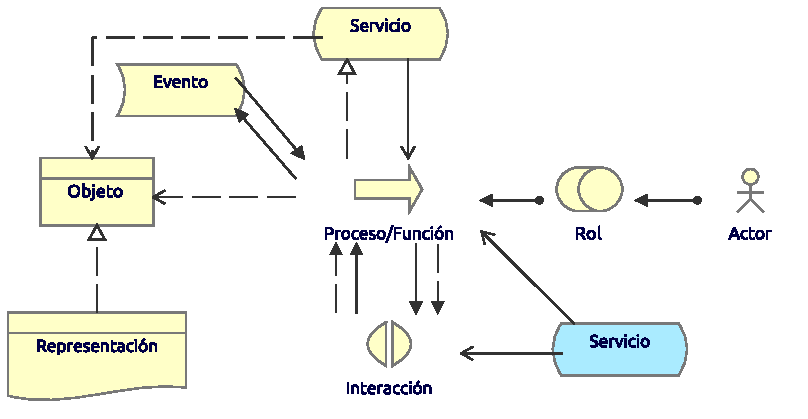
\includegraphics[width=.8\linewidth]{imgs/modelo/ProcesoNegocio}
	\caption{Modelo Proceso de Negocio}
\end{figure}

Un proceso empresarial representa una secuencia de comportamientos empresariales que logra un resultado específico, como un conjunto definido de productos o servicios empresariales.
Un proceso de negocios describe el comportamiento interno realizado por un rol de negocios que se requiere para producir un conjunto de productos y servicios. Para un consumidor, los productos y servicios son relevantes y el comportamiento requerido es meramente una caja negra, de ahí la designación "interno".
Un proceso comercial complejo puede ser una agregación de otros procesos de grano más fino. A cada uno de ellos se le pueden asignar funciones más finas.
Existe una relación potencial de muchos a muchos entre los procesos de negocios y las funciones de negocios. En términos informales, los procesos describen algún tipo de "flujo" de actividades, mientras que las funciones agrupan las actividades según las aptitudes, los conocimientos, los recursos, etc. requeridos. Un proceso empresarial puede ser desencadenado por, o desencadenar, cualquier otro elemento de comportamiento empresarial (por ejemplo, un acto empresarial, un proceso empresarial, una función empresarial o una interacción empresarial). Un proceso empresarial puede acceder a objetos empresariales. Un proceso empresarial puede realizar uno o más servicios empresariales y pueden utilizar servicios comerciales (internos) o servicios de aplicación. Se puede asignar una función empresarial a un proceso empresarial para realizar este proceso manualmente. Un proceso empresarial automatizado puede realizarse mediante un proceso de aplicación. El nombre de un proceso empresarial debe indicar claramente una secuencia predefinida de acciones, y puede incluir la palabra "proceso". Ejemplos de ello son "adjudicar la reclamación", "incorporación de empleados", "proceso de aprobación" o "presentación de informes financieros". \\

Un objeto comercial representa un concepto utilizado dentro de un dominio comercial determinado. Un contrato representa una especificación formal o informal de un acuerdo entre un proveedor y un consumidor en el que se especifican los derechos y obligaciones asociados a un producto y se establecen parámetros funcionales y no funcionales para la interacción. Una representación representa una forma perceptible de la información que lleva un objeto comercial.

\clearpage
\subsection{Caso  de Proceso de Negocio}
\begin{figure}[h!]
	\centering
	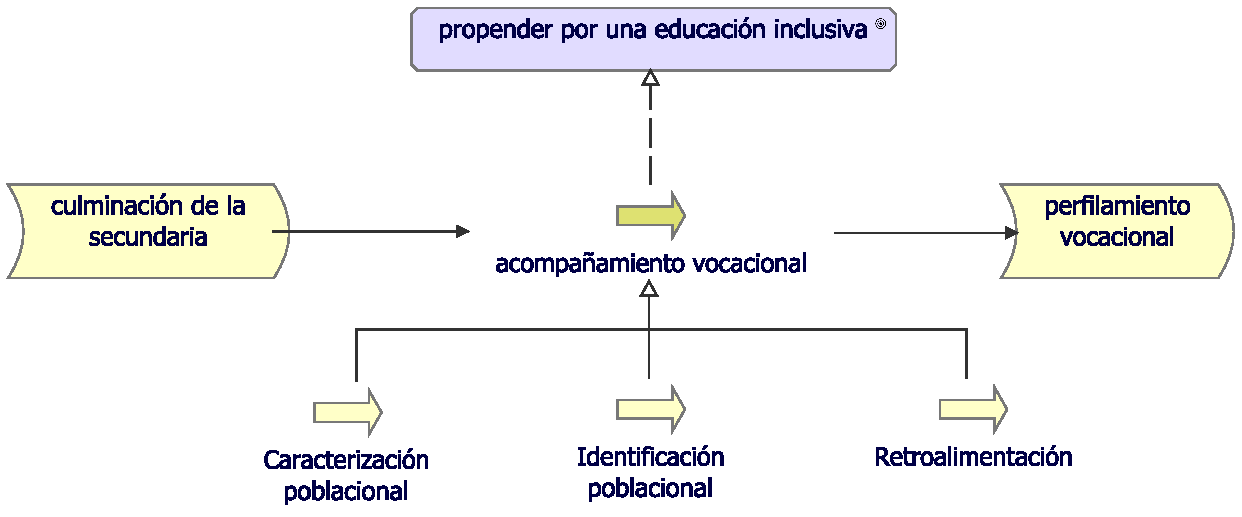
\includegraphics[width=.9\linewidth]{imgs/caso/negocio/proceso}
	\caption{Caso Proceso de Negocio}
\end{figure}

Después de efectuar una revisión documental sobre los procesos del MEN dispuestos para dar alcance a uno de sus principales objetivos, propender por una educación inclusiva, desde nuestra organización proponemos la inclusión de un nuevo proceso capaz de fortalecer y afianzar en la sociedad, ese objetivo de carácter político que conlleve a una educación inclusiva eficiente en cuanto al desarrollo personal y profesional de la comunidad se refiere. Asimismo, este proceso novedoso en el marco actual de la organización, se especializa en tres procesos de carácter secuencial dispuestos de la siguiente manera, una caracterización poblacional, una Identificación poblacional posterior, y finalmente, una retroalimentación individualizada para cada estudiante que culmina la secundaria, evento inicial de nuestro proceso de acompañamiento vocacional, el cual culmina con el perfilamiento vocacional de cada uno de estos estudiantes.



\clearpage
\section{Punto de Vista de Cooperación de Proceso de Negocio}

El punto de vista de cooperación de proceso de negocio, promueve la identificación y asociación de roles a través de procesos, en otras palabras, es la vinculación existente entre los procesos y los roles, este punto de vista se deriva directamente del punto de vista de proceso de negocio y al identificar estos roles, permite expandir la forma en que se entiende el proyecto, asignando responsables a procesos.

\subsection{Modelo de Cooperación de Proceso de Negocio}
\begin{figure}[h!]
	\centering
	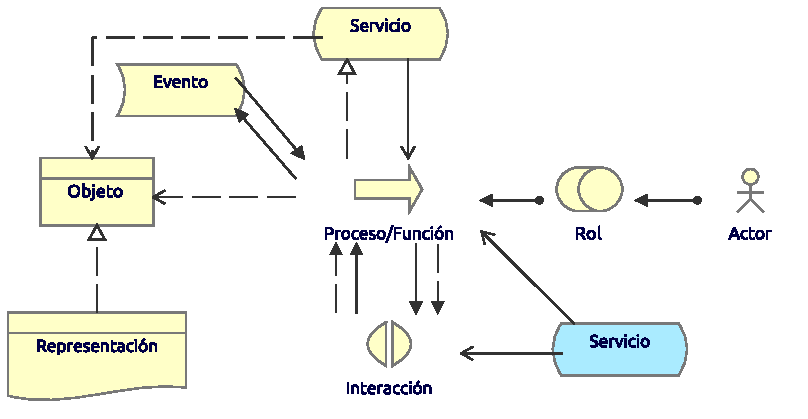
\includegraphics[width=.8\linewidth]{imgs/modelo/ProcesoNegocio}
	\caption{Modelo Cooperación de Proceso de Negocio}
\end{figure}

El modelo del punto de vista de Cooperación de Proceso de Negocio, se compone de un conjunto de partes, principalmente mencionadas en la parte exclusiva del proceso de negocio como lo son: el proceso o función, el evento, los derivados de este evento y proceso como el servicio, el objeto, la interacción y la representación y sin dejar de lado el enlace principal con el proceso el cual es el objetivo, estas partes componen tanto al punto de vista de proceso de negocio como al punto de vista de cooperación de proceso de negocio, a excepción que este segundo punto de vista incluye uno o varios roles, el cual se le asigna al proceso en cuestión.

\clearpage
\subsection{Caso de Cooperación de Proceso de Negocio}
\begin{figure}[h!]
	\centering
	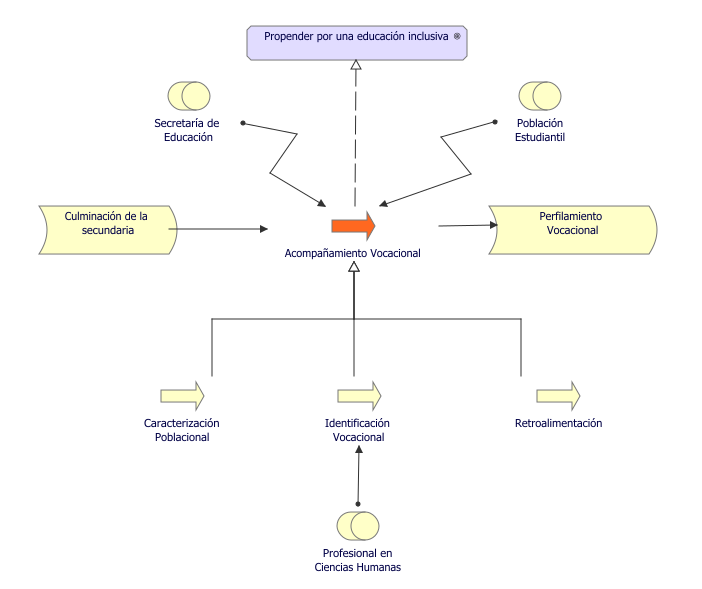
\includegraphics[width=.9\linewidth]{imgs/caso/negocio/CoopProNegocio}
	\caption{Caso Cooperación de Proceso de Negocio}
\end{figure}

Este proyecto de colaboración con el Ministerio de Educación Nacional para tener una educación inclusiva y contribuir con el mejoramiento de la educación en el territorio nacional, posee un gran objetivo el cual es el propender por una educación inclusiva, del cual se deriva el proceso principal de tener un acompañamiento vocacional que lo antecede el evento de negocio de la culminación de la secundaria y lo precede el evento del perfilamiento vocacional, a este gran proceso se le asignan dos roles que intervienen en el, como lo son: la secretaría de educación y la población estudiantil además, este proceso principal cuenta con tres sub procesos: la caracterización poblacional, la identificación vocacional que está vinculada con el rol de los profesionales en ciencias humanas y el subproceso de la retroalimentación.



\clearpage
\section{Punto de Vista de Producto}


\subsection{Modelo de Producto}
\begin{figure}[h!]
	\centering
	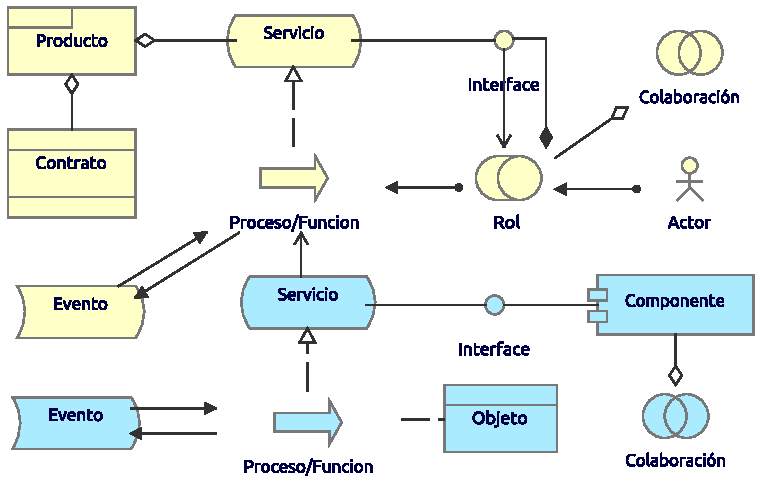
\includegraphics[width=.6\linewidth]{imgs/modelo/Producto.pdf}
	\caption{Modelo Producto}
\end{figure}

El punto de vista de producto permite ver el conjunto de contratos que rigen un producto de la organización, además relaciona los servicios que se desprenden del producto. Estos contratos son aquello que regulan y limitan  al producto. Los servicios asociados al producto son parte de los objetivos, misión y visión de la empresa y que desembocan en proceso de la organización ya sea implícito o explícito relacionado obviamente con el producto.

\newpage
\subsection{Caso  de Producto}
\begin{figure}[h!]
	\centering
	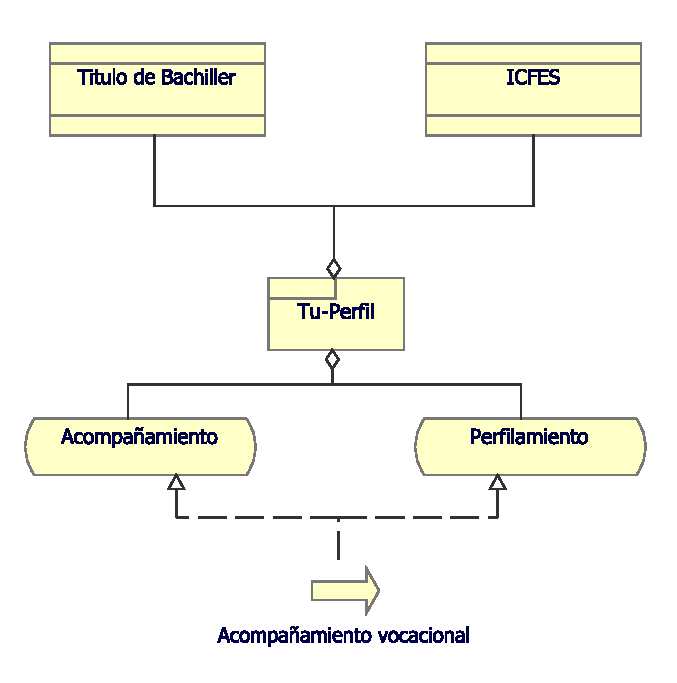
\includegraphics[width=.9\linewidth]{imgs/caso/negocio/producto.pdf}
	\caption{Caso Producto}
\end{figure}

Para el caso de estudio tenemos como producto de negocio a Tu-Perfil aquel apartado que servirá como guiá para acompañar y perfilar a los estudiantes en la elección de vocación que sera tomada al graduarse como bachiller con el fin de dar cabida al proceso de acompañamiento vocacional que surge de los objetivos de la organización para este caso el MEN.  Este producto esta regido por los contratos definidos ICFES y Titulo de Bachiller, que serán aquellos que limitaran al producto.
